% \documentclass{article}

% % Language setting
% % Replace `english' with e.g. `spanish' to change the document language
% \usepackage[english]{babel}

% % Set page size and margins
% % Replace `letterpaper' with `a4paper' for UK/EU standard size
% \usepackage[letterpaper,top=2cm,bottom=2cm,left=3cm,right=3cm,marginparwidth=1.75cm]{geometry}

% % Useful packages
% \usepackage{amsmath}
% \usepackage{graphicx}
% \usepackage[colorlinks=true, allcolors=blue]{hyperref}
% \usepackage{tikz}
% \usepackage{}
% \title{Thesis preliminaries}
% \author{Jordan Moncrieff}

% \begin{document}
% \maketitle

% \begin{abstract}
% In this document, we
% will give a brief introduction to general relativity, black holes, and some plasma Physics\footnote{The Plasma notes where just taken when I was first learning the basics of Plasma Physics, it is unlikely I will add them into the thesis. Also, there are likely mistakes and missing info, as I wrote very quickly.}. Parts of this document could be added into the thesis, although it is far from finished, containing lots of missing information and mistakes.

% \end{abstract}

\chapter{Thesis preliminaries}

\section{Introduction}

Black holes are astronomical bodies that have an escape velocity at the surface greater than the speed of light. A consequence of this, is that anything crosses a certain region called the \textbf{event horizon} of the black hole can not escape. 

Black holes do not make sense in classical Physics perspective, since light in classical mechanics is not affected by classical gravity. Thus we need to understand a subject called \textbf{General Relativity}, which explains the motions of objects in space and time, as a result of the geometry of \textbf{spacetime}, with this geometry being the result of massive objects existing in this spacetime (i.e. planets, stars, humans etc.). 

Throughout this document, we will first give a brief introduction to general relativity (GR) in section \ref{sec:Intro to GR}, followed by a a discussion of how black holes emerge from GR in section \ref{sec:BH soln}. After this introduction, we will then introduce some concepts in plasma physics, also relevant for the thesis. Equations will be given throughout, but they will just be stated and described intuitively. For a more rigorous introduction to GR, their are many great texts introductory texts \cite{carroll2019spacetime, hartle2003gravity}, as well as more rigorous treatments \cite{wald2010general}.

\section{Introduction to general relativity}\label{sec:Intro to GR}

General relativity can be summed up with the quote of John Wheeler, "Spacetime tells matter how to move; matter tells spacetime how to curve". This introduction to GR section will explain this statement in slightly more detail.

GR is built on the notion of spacetime. Spacetime is what you get when you combine space and time into a single unifying object. In order to describe an event, such as the birth of a child, you need to describe both its location in space (which hospital), and when in time the event occurred (the birthday). Thus, events can be parameterized by four numbers (t, x, y, z), called a \textit{world point}. This space then needs a definition of distance between two events in spacetime. This notion of distance should match our intuition of distance in (Euclidean) space for two events located at the same point in time, i.e. the Pythagorean theorem 
$s^2 = \Delta x^2 + \Delta y^2 + \Delta z^2$. But we need to involve time in some way, in flat spacetime, the arena of \textit{special relativity}, the distance between two events $(t_1,x_1,y_1,z_1)$ and $(t_2,x_2,y_2,z_2)$, is given by the \textit{metric} s, given by 

\begin{equation}\label{eq:Flat spacetime metric}
    s^2 = - (t_1-t_2)^2 + (x_1-x_2)^2 + (y_1-y_2)^2 + (z_1-z_2)^2
\end{equation}

Notice that there is a negative in front of the time contribution, this means distance in spacetime is not the same as distance in a general Euclidean space, so our intuition about distance in space does not exactly carry over to spacetime. This leads to many of the non-intuitive concepts of special and general relativity. The reason the metric is chosen in this way, is because all observers will agree on these distances, no matter where observers are or how they are moving. In general relativity, the metric changes in the presence of masses, i.e. distances between points is no longer the flat space distance, and therefore, the straightest path between two points is no longer a straight line.


\begin{figure}
    \centering
    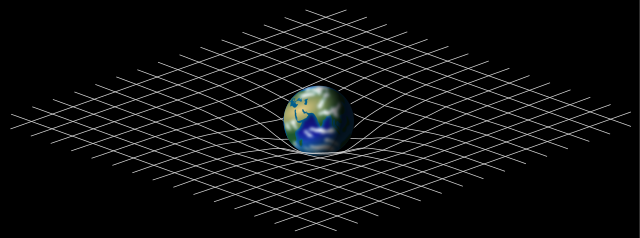
\includegraphics[width=\textwidth]{preliminaries/preliminaries_images/640px-Spacetime_lattice_analogy.svg.png}
        \caption{General relativity illustration - credit NASA}
    \label{fig:GR_analogy}
\end{figure}

General relativity describes gravity as the result of mass curving spacetime, and the resulting curved spacetime causing particles to be deflected along there trajectory toward the mass - manifesting as the attractive Newtonian force we see in the classical world. So anything with mass, in fact anything with energy\footnote{Since by Einstein's mass energy equivalence, anything with energy has mass, and vice-versa.} causes spacetime to curve, as shown in the illustration of in figure \ref{fig:GR_analogy}. Then, any other object with energy within that spacetime will travel in straight lines across this spacetime, resulting in for example orbital motion. 

The way we precisely calculate how energy curves this spacetime, and how particles respond to this curvature, is with the \textit{Einstein field equations} (EFEs).

\begin{equation}
    G_{\mu \nu} + \Lambda g_{\mu \nu} = \kappa T_{\mu \nu}
\label{eq:EFE}
\end{equation}

Where 

\begin{itemize}
    \item $G_{\mu \nu}$ is the Einstein tensor, representing the curvature of space-time.
    
    \item $T_{\mu \nu}$ is the stress energy tensor, representing the density and flux of energy/momentum in space-time.
    
    \item $\Lambda$ is the cosmological constant, which gives rise to the accelerating expansion of the universe.
    
    \item $\kappa=\frac{8\pi G}{c^4}$ is a constant.
    
    \item $g_{\alpha \beta} = \boldsymbol{e}_\alpha \cdot \boldsymbol{e}_\beta$ is the metric tensor, given by the dot product of the basis vectors, and $g^{\alpha \beta}$ is the inverse metric tensor. The metric tensor allows for measurements of distance in space-time, and can be thought of as representing the gravitational field in general relativity.
 \end{itemize}


The Einstein tensor can be written as

\begin{equation}
    G_{\mu \nu } = R_{\mu \nu} - \frac{1}{2} R g_{\mu \nu}
\label{eq:Einstein tensor}
\end{equation}

Where the R tensor are contractions of the Ricci tensor defined by equation 

\begin{equation}
    R_{\sigma \mu \nu }^{\rho }=\partial_{\mu} \Gamma _{\nu \sigma }^{\rho }-\partial_\nu \Gamma _{\mu \sigma }^{\rho }+\Gamma _{\nu \sigma }^{\lambda } \Gamma _{\mu \lambda }^{\rho }-\Gamma _{\mu \sigma }^{\lambda } \Gamma _{\nu \lambda }^{\rho }
\label{eq:Riemann tesnor}
\end{equation}


\begin{itemize}
    \item $R_{\mu \nu} = R^{\alpha}_{\nu \alpha \beta}$ is the Ricci curvature tensor, which roughly represents how much the curved space-time deviates from flat space-time.
    \item R = $R^{\alpha}_{\alpha}$ is the Ricci scalar, the contraction of the Ricci tensor, a measure of curvature.
\end{itemize}

And gamma coefficients $\Gamma^{\mu}_{\nu \sigma}$ describes the Christoffel symbols (or affine connection), which itself is given by the formula

\begin{equation}
    \Gamma^{\mu}_{\nu \sigma} = \frac{1}{2} g^{\alpha \mu} (\partial_{\nu}g_{\alpha \sigma}+\partial_{\sigma} g_{\nu \alpha} - \partial_{\alpha} g_{\nu \sigma})
\label{eq:Christoffel symbol}
\end{equation}

These gamma coefficients represent how basis vectors change between points in space.

TODO: Go more into the intuition behind the terms in the EFEs.

\subsection{Derivation of EFEs from action}

TODO: Derive the Einstein field equations from the Einstein-Hilbert action. Also motivate the action (along with the field equations) by considering the basic principles of general relativity (i.e. the strong equivalence principle, principle of general covariance). Also describe some basics of differential geometry.


\section{Black hole solutions}\label{sec:BH soln}

Black holes are simultaneously extremely complicated, and yet incredibly simple. The complexity comes from the difficulty of solving Einstein's field equations, the simplicity comes from a result known as the "No hair theorem". The no hair theorem states that black holes are completely characterised by three parameters, the mass M, the spin J, and the charge Q. These free parameters give rise to different types of black holes.

\begin{enumerate}
    \item Schwarzschild Black Holes: The Schwarzschild black hole is the simplest and most fundamental black hole solution. It is spherically symmetric and has no spin or charge (J = 0, Q = 0). The mass parameter M is the only defining characteristic of a Schwarzschild black hole. It is surrounded by an event horizon, beyond which gravity is so intense that nothing, not even light, can escape. 
    \item Kerr Black Holes: The Kerr black hole is characterized by both mass and angular momentum or spin (J ≠ 0). It possesses a rotating singularity and an event horizon known as the ergosphere, which is larger than the event horizon of a Schwarzschild black hole. The rotation of a Kerr black hole introduces frame-dragging effects, where spacetime itself is dragged along with the rotating black hole. These effects have profound implications for phenomena such as accretion disks, jets, and the extraction of energy from black holes through processes like the Penrose process. Kerr black holes are the most astrophysically relevant of the black hole solutions, as all black holes in nature are expected to be Kerr black holes.
    \item Reissner-Nordström Black Holes: The Reissner-Nordström black hole incorporates electric charge (Q ≠ 0) along with mass (M) and has no spin (J = 0). Electrically charged black holes are relatively theoretical, as astrophysical objects are typically electrically neutral. However, they play a crucial role in understanding the interplay between gravity and electromagnetism. The presence of charge alters the structure of the event horizon and affects the behavior of charged particles near the black hole. Reissner-Nordström black holes provide insights into the behavior of charged matter falling into a black hole and are crucial in studies involving the cosmic censorship hypothesis.
    \item Kerr-Newman  black holes: The Kerr-Newman black hole extends the Kerr black hole solution by incorporating both mass, angular momentum (spin), and electric charge (J ≠ 0, Q ≠ 0). Like Reissner-Nordström black holes, they are not expected to be Astrophysically relevant.
\end{enumerate}


\subsection{Schwarzschild metric}

The distance between two points in space-time is given by the invariant line element $ds^2$. In Schwarzschild space-time, the line is given by equation (\ref{eq:Schwarzschild line-element}) (given in units c=1).

\begin{equation}
    ds^2 = - d\tau^2 = - (1-\frac{2 G M}{r}) dt^2 +  (1-\frac{2 G M}{r})^{-1} dr^2
            + r^2 (d\theta^2+\sin^2\theta d\phi^2)
\label{eq:Schwarzschild line-element}
\end{equation}

I derived the Schwarzschild metric in schwarzschild\_solution.nb, a Mathematica notebook based on the OGRe Mathematica package \cite{Shoshany2021_OGRe} for GR calculations.

\subsection{Kerr metric}

The metric for a Kerr black hole (spherically symmetric, stationary, black hole of mass M rotating at constant angular momentum J) is given by (in units G=c=1)

\begin{equation}\label{eq:Kerr metric}
    ds^2 = -\left(1-\frac{2Mr}{\rho^2}\right) dt^2-\frac{4Mar \sin^2{\theta}}{\rho^2} d\phi dt+ \frac{\rho^2}{\Delta} dr^2 + \rho^2 d\theta^2 +\left(r^2+a^2+
    \frac{2Mra^2\sin^2{\theta}}{\rho^2}
    \right)\sin{\theta}^2 d\phi^2
\end{equation}

Where $a:=\frac{J}{M}$, $\rho^2:=r^2+a^2 \cos{\theta}$, and $\Delta:=r^2-2Mr+a^2$ \cite{carroll2019spacetime}.

It is easy to see that setting $a=0$ leaves us with the Schwarzschild solution (the case of zero spin is the same as Schwarzschild solution in equation (\ref{eq:Schwarzschild line-element})), and in the limit that $r \gg a$ we get the weak field metric (in terms of gravitational potential $\Phi(r)=-\frac{G M}{r}$)

\begin{equation}
    ds^2 = - (1+2\Phi(r)) dt^2 +  (1-2\Phi(r)) dr^2
            + r^2 (d\theta^2+\sin^2\theta d\phi^2)
\label{eq:Weak field metric}
\end{equation}

Which as $r\rightarrow \infty$ approaches flat (Minkowski) spacetime

\begin{equation}
    ds^2 = - dt^2 + dx^2 + dy^2 + dz^2
\label{eq:Minkowski metruc}
\end{equation}

\subsection{Reissner–Nordström metric}
\begin{equation}
    ds^2 = -\left(1 - \frac{{2GM}}{{r}} + \frac{{GQ^2}}{{r^2}}\right)dt^2 + \left(1 - \frac{{2GM}}{{r}} + \frac{{GQ^2}}{{r^2}}\right)^{-1}dr^2 + r^2(d\theta^2 + \sin^2\theta d\phi^2)
\end{equation}

where G is the gravitational constant, M is the mass of the black hole, Q is its electric charge, and (t,r,θ,ϕ) are the coordinates in the metric.

\subsection{Kerr-Newman}

\section{Orbits of Black holes}\label{sec:Orbits}

See black hole orbits document.

\section{Gravitomagnetism}\label{sec:Gravitomagnetism}

\subsection{Gravitomagnetic equations}

TODO - Derivation of gravitmagnetic equations from weak field limit of general relativity.

\begin{align}\label{eq:Gravitomagnetic equations}
    \nabla \cdot \mathbf{E_g} &= - 4\pi G \rho_g \\
    \nabla \times \mathbf{E_g} &= - \frac{\partial \mathbf{B_g}}{\partial t}\label{eq:Gravitomag grad E} \\
    \nabla \cdot \mathbf{B_g} &= 0 \\
    \nabla \times \mathbf{B_g} &= - \frac{4\pi G}{c^2} \mathbf{J} + \frac{1}{c^2} \frac{\partial \mathbf{E_g}}{\partial t}\label{eq:Gravitomag Partial E}
\end{align}

Where $\mathbf{E_g}$ is the gravito-electric field, $\mathbf{B_g}$ is the gravitomagnetic field, and $\rho_g$ is the mass density. Almost identical to Maxwell's equations in equations (\ref{eq:Maxwells}).



\subsection{Frame dragging}

% \begin{tikzpicture}

% % Draw sphere
% \shade[ball color=blue!10!white,opacity=0.7] (0,0) circle (2cm);

% % Draw equator
% \draw[dashed] (0,0) circle (2cm);


% % Draw charge density
% \foreach \i in {0,45,...,360} {
%   \filldraw[fill=white,draw=black] (\i:1.5cm) circle (0.2cm) node[blue!70!black] {$+$};
%   \filldraw[fill=white,draw=black] (\i:0.5cm) circle (0.2cm) node[blue!70!black] {$+$};
% }

% \draw ((3*0.71,3*0.71) .. controls (3*1,0)  .. (3*0.71,- 3*0.71);)

% \draw[blue, directed] (3*cos(30), 3*sin(30)) ellipse (3*cos(-30), 3*sin(-30))



% % % Indicate positive charges
% % \node[blue!70!black] at (0,1.8) {$+$};
% % \node[blue!70!black] at (0,-1.8) {$+$};

% % Draw magnetic field lines
% \foreach \i in {0,30,...,360} {
%   \draw[->,thick,green!70!black] (\i:2.2cm) -- (\i:3.5cm);
% }

% \draw[ultra thick, ->] (-3,-1.5) arc (220:320:4)

% \draw[ultra thick, ->] 


% \end{tikzpicture}


Imagine a charged sphere rotating about its axis. The rotating charges will form current loops, and hence an electric dipole will be generated. This electric dipole will exert effectively a magnetic force on an incoming charged particle, with the direction given by the right hand rule. Consider now, the analogous gravitational situation, i.e. a sphere of matter rotating about its axis. The rotation of the mass will result in a gravitomagnetic force acting on an incoming moving mass, this is known as the Lens-Thirring effect, and has been experimentally verified. This situation resembles very well the concept of frame dragging, a black hole rotating drags spacetime with it, and indeed the direction of the force from frame dragging can be found by using the right hand rule.


\section{Magnetohydrodynamics}\label{sec:Magnetohydrodynamics}

Magnetohydrodynamics (MHD) is the study of magnetic fields in conductive fluids, hence it is a combination of fluid mechanics with electromagnetism. In this section, we will cover the minimum amount of MHD theory necessary to understand magnetic reconnection. The reference used for all of this is the text "The Physics of Fluids and Plasmas, An Introduction for Astrophysicists" by ARNAB RAI CHOUDHURI \cite{choudhuri_1998}.

\subsection{Fluid mechanics and Navier-Stokes equation}
Fluid mechanics is governed by the Navier-stokes equation

\begin{equation}\label{eq:Navier-Stokes}
    \underbrace{\frac{D \Vec{v}}{Dt}}_{\text{Acceleration}} = 
    \underbrace{\Sigma_{i}\Vec{F_i}}_{\text{External forces}} - 
    \underbrace{\frac{1}{\rho} \nabla p}_{\text{Pressure gradient}} + 
    \underbrace{\nu \nabla^2 \Vec{v}}_{\text{Viscosity}}
\end{equation}

Where the left hand side is the Lagrangian derivative, which is just the full derivative of the velocity field of the fluid 
$\Vec{v}(t,\Vec{x})$ obtained by using the chain rule


\begin{equation}
    \frac{D\Vec{v}}{Dt} := \frac{d\Vec{v}}{dt} = \frac{\partial \Vec{v}}{\partial t} + (\Vec{v}\cdot\nabla)\Vec{v}
\end{equation}

Which we can see comes with a contribution from the time dependence through the partial with respect to t, as well as the directional derivative of the velocity field in the direction of the velocity. Hence, the total derivative represents the change in the velocity of the fluid after an infinitesimal step in time accompanied by an infinitesimal step in the direction of the fluid velocity. This means intuitively, the total derivative, which is also called the material derivative in fluid mechanics, is the rate of change of fluid velocity according to an observer moving with the fluid flow at a point. So, the left hand side describes an acceleration. Hence, by Newton's second law, the right hand side represents a force (divided by mass, and divided by volume since we are only considering an infinitesimal fluid element with a given density). The first term on the right hand side represents external forces applied to the fluid, such as gravity, electric fields etc. The next term is the acceleration due to a pressure gradient, since pressure is force divided by area acting in all directions at a point, if there is a difference in pressure between two points (a pressure gradient) there will be a net force accelerating any object in the direction opposite the pressure gradient. The final term represents viscocity, which is essentially how hard it is to move through the fluid. Note that viscosity is represented by a difussion term, similar to heat in the heat wquation. This term represents the diffusion of velocity within the fluid. To see why this makes sense, consider that a difference in velocity of a fluid element compared to its negibours (given by the laplacian of the velocity field) will result in the element giving some of its velocity to its neighbours due to frictional effects caused by its viscosity. This has the result of spreading the velocity out through the fluid, exactly like a classic diffusion process. 

The Navier-Stokes equation applies 

% \begin{equation}
%     \nabla \cdot \Vec{B} = 0 \\
%     \nabla x \Vec{E} = -\frac{1}{c} \frac{\partial \Vec{B}{\partial t} = 0 \\
%     \nabla 
% \end{equation}

\subsection{Electromagnetism}

Electromagnetism is governed by the Maxwell equations, given below in Gaussian-cgs units

\begin{align}\label{eq:Maxwells}
    \nabla \cdot \mathbf{E} &= 4\pi\rho \\
    \nabla \times \mathbf{E} &= -\frac{1}{c} \frac{\partial \mathbf{B}}{\partial t}\label{eq:Maxwell grad E} \\
    \nabla \cdot \mathbf{B} &= 0 \\
    \nabla \times \mathbf{B} &= \frac{4\pi}{c} \mathbf{J} + \frac{1}{c} \frac{\partial \mathbf{E}}{\partial t}\label{eq:Maxwell Partial E}
\end{align}

where $\rho$ is the charge density, $\mathbf{J}$ is the current density, $\mathbf{E}$ is the electric field, $\mathbf{B}$ is the magnetic field, and $c$ is the speed of light. Note that Gaussian-cgs (centimeters, grams, seconds) units are used in the above equations in order to get rid of the nonphysical factor $k=\frac{1}{4\pi \epsilon_0}$ in the electrostatic force law. Setting $k=1$ gives the simpler $\Vec{F} = \frac{q_1 \cdot q_2}{r^2}$, which is done in Gaussian-cgs units. In this new coordinate system we now use the unit of charge called the electrostatic unit (esu), force has the unit dyne, energy ergs, etc\footnote{Fill this out with more detail later}.

% \begin{itemize}
%     \item \frac{D}{Dt} = \frac{\partial \Vec{v}}{\partial t} 
%     % := \frac{d\Vec{v}{dt} = \frac{\partial \Vec{v}}{\partial t} 
% \end{itemize}

\subsection{Magnetohydrodynamics basic equation}

We get the basics of Magnetohydrodynamics by combining the equations of fluid dynamics with Maxwell's equations, which leads to various new phenomena. For example, by adding a Coulomb force term, from equation \ref{eq:Navier-Stokes}

\begin{equation}\label{eq:Navier-Stokes added in Coulomb}
    \frac{\partial \Vec{v}}{\partial t} + (\Vec{v}\cdot\nabla)\Vec{v} = 
    \Sigma_{i}\Vec{F_i} - 
    \frac{1}{\rho} \nabla p + 
    \frac{1}{\rho c} \Vec{J} \times \Vec{B} +
    \nu \nabla^2 \Vec{v}
\end{equation}

But from equation \ref{eq:Maxwell grad E}, when setting the displacement current 
$\frac{1}{c} \frac{\partial \Vec{E}}{\partial t} ~ \frac{v^2}{c^2} = 0$, and using the vector product identity

\begin{equation}\label{Vector identity curl B curl B}
    (\nabla \times \Vec{B}) \times \Vec{B} = (\Vec{B} \cdot \nabla) \Vec{B} - \nabla (\frac{B^2}{2})
\end{equation}

We arrive at the analogous Navier-Stokes equation for Magnetohydrodynamics

\begin{equation}\label{eq:Navier-stokes for MHD}
    \underbrace{\frac{\partial \Vec{v}}{\partial t} + (\Vec{v}\cdot\nabla)\Vec{v}}_{\text{Acceleration}} = 
    \Sigma_{i}\Vec{F_i} - 
    \frac{1}{\rho} \nabla \underbrace{ \left( p + \frac{B^2}{8 \pi} \right)}_{\text{Effective pressure}} + 
    \underbrace{\frac{(\Vec{B}\cdot \nabla) \Vec{B}}{4 \pi \rho}}_{\text{Effective tension}} + 
    \underbrace{\frac{1}{\rho c} \Vec{J} \times \Vec{B}}_{\text{Lorentz force}} +
    \nu \nabla^2 \Vec{v}
\end{equation}

This equation introduces two new phenomenon, one is magnetic pressure, given by $\frac{B^2}{8 \pi}$; and the other is magnetic tension, given by 

\begin{equation}\label{eq:Magnetic tension}
    \Vec{f_T} = \frac{(\Vec{B}\cdot \nabla) \Vec{B}}{4 \pi}
\end{equation}

\subsection{Magnetic pressure}

Magnetic pressure is $B^2/8\pi$. If there is a magnetic field gradient, so region with stronger magnetic field has a greater pressure then neighbouring region, there will be a net force on the particles pushing the plasma from the high magnetic field region to the lower magnetic field region.

To see where this comes from, imagine charged particles in plasma moving along a magnetic field line, in helical motion. If the magnetic field strength is weaker to one side, as the ion spirals towards the lower magnetic field, the Lorentz force back towards the higher B field will be weaker than before, hence the particle will experience a force toward the region with a lower magnetic field – acting exactly like a pressure gradient in a fluid.


\subsubsection{Magnetic tension}

Magnetic tension is a restoring force that acts to oppose curvature in magnetic field lines. It has a magnitude $\frac{B^2}{4\pi}$, and its direction is given by the directional derivative of the magnetic field $\Vec{B}$ in the direction of $\Vec{B}$, hence it points to the centre of curvature of the magnetic field lines\footnote{This is the same as how the acceleration vector of a car passing through a round about points towards the centre of the round about, vector diagram is helpful.}, as shown in figure \ref{fig:Magnetic tension} .

\begin{figure}
    \centering
    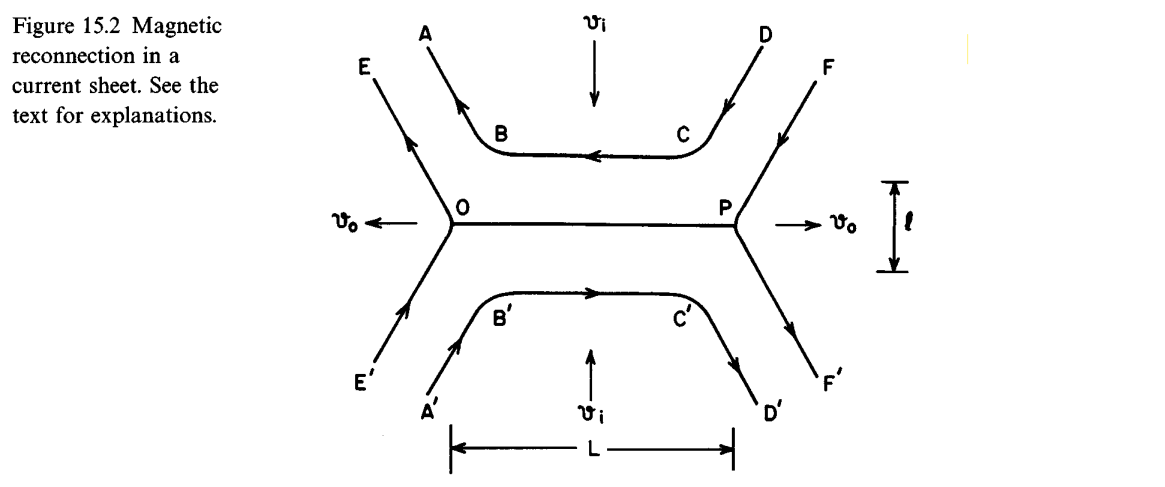
\includegraphics[width=0.5\textwidth]{preliminaries/preliminaries_images/magnetic_reconnection.png}
    \caption{Illustration of magnetic tension, which acts to straighten magnetic field lines. $\kappa$ is the reciprocal of the radius of curvature. This was taken by the \href{https://en.wikipedia.org/wiki/Magnetic_tension}{wikipedia article} on magnetic tension, which is decent.}
    \label{fig:Magnetic tension}
\end{figure}

\subsubsection{Energy equation}
From the Maxwell equation \ref{eq:Maxwell Partial E}, for the electric field in the moving reference frame of a plasma with velocity $\Vec{v}$ given by 

\begin{equation}\label{eq:Electric field in moving frame}
    \Vec{E} = -\Vec{v} \times \Vec{B}
\end{equation}

We can arrive at the induction equation

\begin{equation}\label{eq:Induction equation}
    \frac{\partial \Vec{B}}{\partial t} = \nabla \times (\Vec{v} \times \Vec{B}) + \lambda \nabla^2 \Vec{B}
\end{equation}

Where $\lambda = \frac{c^2}{4 \pi \sigma}$ is the magnetic diffusivity. When the conductivity $\sigma$ is very high (infinite in ideal case), the diffusion term is negligible (this is the case for most plasma's). However, this diffusion leads to damping of magnetic fields in relatively low conducting plasma regions, which is important for magnetic reconnection. This magnetic damping becomes important when the magnetic Reynolds number is sufficiently small.

\subsubsection{Magnetic Reynolds number}

The magnetic Reynolds is a dimensionless number defined in terms of the length scale of the system $L$, typical velocity scale $V$, typical magnetic field $B$, and diffusivity $\lambda$. It can be found by making equation \ref{eq:Induction equation} dimensionless by scaling the variables. Rewriting all quantities in terms of dimensionless form, $\Vec{B} = B\Vec{B}^'$, $\Vec{v} = V \Vec{v}^'$, and $\nabla=\nabla'$, we get 

% \begin{align}
%     \frac{\partial (B \Vec{B}^{'})}{\partial t} &= 
%     \nabla \times (V \Vec{v}^{'}) \times ( B \Vec{B}^{'})) + 
%     \lambda \nabla^2 (B \Vec{B}^{'}) \\
    
%     % B \frac{\partial \Vec{B}^{'})}{\partial t} &= 
%     % V B\nabla \times (\Vec{v}^{'}) \times (\Vec{B}^{'})) + 
%     % B \lambda \nabla^2 (\Vec{B}^{'}) \\

%     % \frac{\partial \Vec{B}^{'})}{\partial t} &= 
%     % V B\nabla \times (\Vec{v}^{'}) \times (\Vec{B}^{'})) + 
%     % B \lambda \nabla^2 (\Vec{B}^{'}) \\

% \end{align}

And thus we identify the dimensionless quantity

\begin{equation}\label{eq:Magnetic Reynolds number}
    R_M = \frac{V B/L}{\lambda B / L^2} = \frac{L V}{\lambda}
\end{equation}

The magnetic Reynolds number is analogous the the Reynolds number from fluid dynamics. In fluid dynamics, the Reynolds number is the same for fluid flows around geometrically similar objects, so experiments can be done at smaller scales to determine dynamics. The Reynolds number also determines the relative importance of the nonlinear behavior, and hence characterises whether a flow will be laminar (simple) or turbulent (complicated and hard to predict). 

For small $R_m$, the field will diffuse away, smoothing out across space. For large $R_m$, the field will remain frozen into the fluid, moving along with the plasma flow.

\subsection{Alfven's theorem and flux freezing}

A very important concept in MHD is Alfven's theorem. Which states that in ideal MHD (i.e. where the fluids are a perfect electrical conductor, such that resistance is infinite and there are no electric fields) magnetic fields in the conducting fluid are constrained to move with the fluid, and the fluid is constrained to move with the magnetic field. This means the magnetic fields are "frozen in" to the fluid. 

This theorem only applies in ideal MHD, but is relevant for high magnetic Reynolds numbers $R_m$. (Explain what the magnetic Reynolds number is, bring up analogy with vorticity and Kelvins circulation theorem, etc).

Intuitively, Alfven's theorem works as follows: Plasma is a bunch of electrons and ions, so when a magnetic field line moves charged particles experience a force, forcing plasma to move with the moving magnetic field (by Lenz law, charges are opposing change in magnetic flux, hence will maintain their position). Alfen's theorem only holds in the non-relativistic limit, since when magnet moves at v~c there is a non-negligable delay time before the charged particles respond, meaning the particles do not perfectly flow with the field.


\subsection{Alfven waves}

Magnetic tension gives rise to Alfven waves. Alfven waves are analogous to sound waves, but instead of a pertubraiton in pressure travelling, Alfven waves result from a perturbation of the magnetic field in the fluid, and are propagated thanks to the restoring force provided by magnetic tension.

\subsection{Magnetic reconnection}
Thanks to Alfven's theorem, the magnetic topology of an ideal magnetofluid ($R_m=\infty$) is fixed. However, magnetic reconnection relies on the fact that for a region finite resistivity there can be a change in the topology, allowing magnetic field lines to combine, changing the structure of the magnetic field and hence redirecting plasma in potentially highly energetic bursts.

Magnetic field lines combine in locations where the magnetic field gradient is large, and hence overpowering the small value of $\lambda$ in equation \ref{eq:Induction equation} for high conductivity, allowing for "cutting and pasting" of field lines. These regions of large magnetic field gradients must be associated with high currents, and hence are known as current sheets. Outside these current sheets, we can assume Alfven's theorem holds, and hence magnetic topologies are preserved everywhere except for small regions known as current sheets.

\begin{figure}
    \centering
    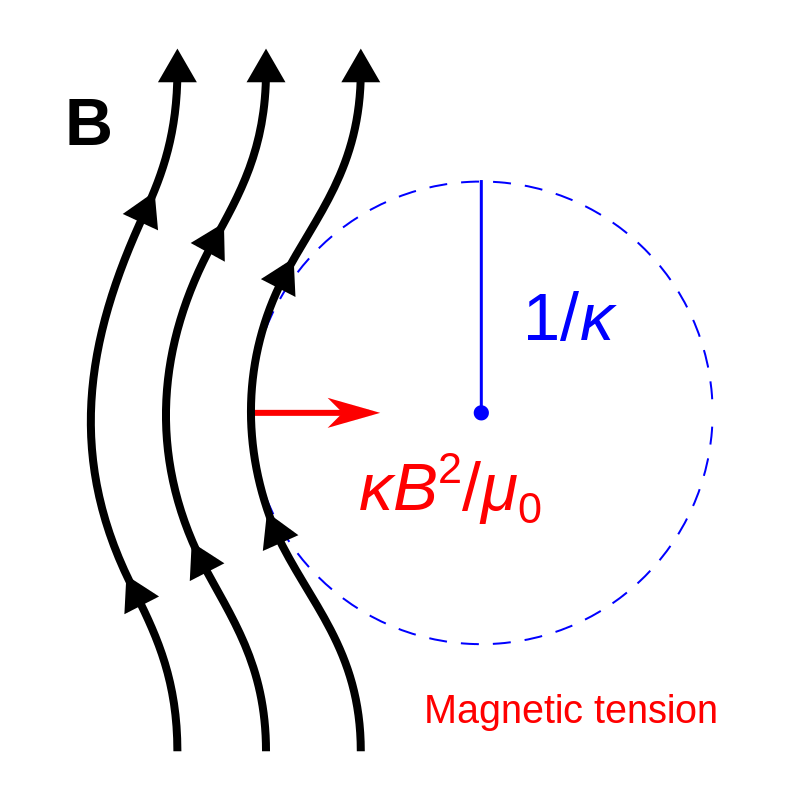
\includegraphics[width=0.5\textwidth]{preliminaries/preliminaries_images/Magnetic_tension_diagram.svg.png}
    \caption{Magnetic reconnection figure, from textbook.}
    \label{fig:Magnetic reconnection, from textbook}
\end{figure}

A current sheet is shown in figure \ref{fig:Magnetic reconnection, from textbook}, where the magnetic field rapidly decreases approaching OP from below, and reaches zero at OP before changing direction and rapdily increasing extending above OP. Due to magnetic pressure being $B^2 / 8\pi$, the pressure above and below the central region is much greater, this will result in plasma from above and below OP to be sucked into the centre, dragging the frozen in flux with it. This magnetic field will then decay according to the induction equation, since in the high magnetic gradient at the centre means the diffusion term in the induction equation become important, resulting in the magnetic field going to zero along the line OP. By conservation of mass, the sucked in plasma must be squeezed out to the left and right, and at this point the magnetic field lines of the originally separated field line travelling from A' to B' will connect with  the line going from  A to B, and likewise C'D' will connect with CD, due to the fact that the horizontal field lines B'C' and BC will have decayed to zero, effectively cutting the horizontal field lines, and pasting the colliding vertical field lines together.

TODO: Condense the plasma discussion, focussing more on physical reasoning than mathematical derivations. Talk more about high energy astro phenomena and applications.



\bibliographystyle{unsrt}
\bibliography{preliminaries/preliminaries_ref}

% \end{document}